\section{Task Evaluation on Temporal Graphs} \label{sec:task}
% \wh{Add some intro. Otherwise, too sudden to start with notation}
% \ah{added intro and explicitly state we focus on continuous time temporal graphs}
\vspace{-8pt}
Temporal graphs are often used to model networks that evolve over time where nodes are entities and temporal edges are relations between entities through time. In this work, we focus on continuous time temporal graphs and denote them as timestamped edge streams consisting of triplets of source, destination, and timestamp; i.e., $\mathcal{G}=\{ (s_0,d_0,t_0), (s_1,d_1,t_1), \dots , (s_T,d_T,t_T) \}$ where the timestamps are ordered (\textit{$0 \leq t_1 \leq t_2 \leq ... \leq t_T $})~\cite{poursafaeitowards,kazemi2020representation}. 
Note that temporal graph edges can have different properties namely being weighted, directed, or attributed. 
We consider $\mathcal{G}_t$ as the augmented graph of all edges observed in the stream up to the time $t$ with nodes as $\mat{V}_t$ and edges as $\mat{E}_t$.
Optionally, $\mathcal{G}_t$ can contain node features $\mat{X}_t \in \mathbb{R}^{|\mat{V}_t| \times k_n}$ where $k_n$ is the size of a node feature vector, and edge features $\mat{M}_t \in \mathbb{R}^{|\mat{E}_t| \times k_m}$ where $k_m$ is the size of an edge feature vector. 
We consider a fixed chronological split to form the training, validation, and test set. 



\textbf{Evaluation Settings.} There are several possible evaluation settings in the temporal graph based on the available information of the test set. 
We categorize and discuss these settings in detail in Appendix~\ref{app:eval}. 
In this work, we consider the \emph{streaming setting} where the deployed models need to adapt to new information at inference time. More specifically, we follow the setting in~\cite{rossi2020temporal} where previously observed test edges can be accessed by the model but back-propagation and weight updates with the test information are not permitted.
%\ah{clarified the motivation for evaluation setting. }

% In this work, we only consider the \emph{streaming setting} information observed during the test phase is available only for updating the memory module\todo{ER: I think that when describing the evaluation settinng we should not describe in terms of specific details of some models, but be more general. I.e. just say that previous test edges can be accessed by the model, but the model cannot update its weights based on them} in several temporal graph learning methods such as TGN~\cite{rossi2020temporal}. 
% It should be noted that in the streaming setting, the test set information is not used for back-propagation and model updates.
% \wh{+1 to Ema's point. Evaluation should be explained based on real-world use-case, not based on models.}


\subsection{Dynamic Link Property Prediction}
% \wh{paragraph too long.}
%defining historical and random edges? 
%In real scenarios, the true edges are not known in advance, thus the top-ranked edges from a given model are often used to decide which connections should be prioritized. In order to capture this in evaluation, it is common to sample a fixed number of negative (or fake) edges per positive (or true) edge. Recently, it has been shown that \emph{historical negatives} are more difficult than random negatives for the models to predict~\cite{poursafaeitowards}. Historical negatives are sampled from the set of edges that were observed in the training set but are not present at the current timestamp $t$ (i.e., $E_{t} \setminus E_\text{train}$).

%In current evaluation~\cite{xu2020inductive,rossi2020temporal,wang2021tcl,souza2022provably,you2022roland}, only one negative edge is sampled uniformly randomly from all possible node pairs~(called \emph{random negatives}) to evaluate against each positive edge. 

The goal of \emph{dynamic link property prediction} is to predict the property~(oftentimes the existence) of a link between a node pair at a future timestamp. 
The timeline is chronologically split at two fixed points resulting in three sets of edges $E_\text{train}$, $E_\text{val.}$, and $E_\text{test}$. In \name, we improve the evaluation setting in the following ways. 

\textbf{Negative edge sampling.} In current evaluation~\cite{kumar2019predicting,xu2020inductive,rossi2020temporal,wang2021tcl,souza2022provably,you2022roland,chanpuriya2022direct,zhou2022tgl}, only one negative edge is sampled uniformly randomly from all possible node pairs to evaluate against each positive edge. 
In contrast, in real applications where the true edges are not known in advance, the edges with the highest probabilities predicted by a given model are used to decide which connections should be prioritized. 
With that in mind, we treat the link prediction task as a ranking problem and sample multiple negative edges per each positive edge. %\todo{ER: Need to explain better the filtering and what collisions are. it's not clear atm}.
\changed{In particular, for a given positive edge $e^p:(s,d,t)$, we fix the source node $s$ and timestamp $t$, and sample $q$ different destination nodes. For each dataset, we select the number of negative edges $q$ based on the trade-off between evaluation completeness and the test set inference time. }

We sample the negative edges from both the \emph{historical} and \emph{random} negative edges. 
Historical negatives are sampled from the set of edges that were observed in the training set but are not present at the current timestamp $t$ (\emph{i.e.} $E_{t} \setminus E_\text{train}$), \changed{they are shown to be more difficult for models to predict than random negatives~\cite{poursafaeitowards}. }
We sample equally from historical and random negative edges. Note that depending on the dataset and the timestamp $t$, there might not be enough historical negatives to sample from. In this case, we simply increase the ratio of the random negatives to have the desired number of negative edges per positive ones.
For reproducibility, we include a fixed set of negatives sampled for each dataset to ensure consistent comparison amongst models.

\textbf{Performance metric.} The commonly used metric for reporting models' performance for the dynamic link prediction task is either Area Under the Receiver Operating Characteristic curve~(AUROC) or Average Precision~(AP). 
An appropriate metric should be able to capture the ranking of a positive edge amongst the negative ones, which is not fulfilled by neither AUROC or AP.
Thus, 
% However, a good metric should capture the ranking of the positive edge amongst the negative ones. Both AUROC and AP are not designed to capture the ranking of the positive edge thus 
% Considering the new approach of sampling negative edges which induces class imbalance, these metrics do not provide an appropriate measure of the actual performance of the models. The higher ranked the probability assigned to the true destination by a given model, the better the MRR metric is.
we devise to use the filtered Mean Reciprocal Rank~(MRR) as the evaluation metric for the dynamic link property prediction. 
The MRR computes the reciprocal rank of the true destination node among the negative or fake destinations. 
% thus, the MRR metric focuses on the rank of the true edge among the negative ones. 
The MRR varies in the range of $(0,1]$ and it is a commonly used metric in recommendation systems~\cite{wu2022graph} and knowledge graphs~\cite{wang2022interht,hu2020open,hu2021ogb}. \changed{In addition, recent link prediction literature is also shifting towards adopting the MRR metric~\cite{chamberlain2022graph,hu2021ogb,yin2022algorithm}.} It should be noted that when reporting the MRR, we perform collision checks to ensure that no positive edge is sampled as a negative edge. 
% Thus, we report the \emph{filtered MRR} indeed. 



%During evaluation of dynamic link prediction, it is important to evaluate the model against both true edges as well as negative edges (or fake edges). 

% \todo[inline]{We should explain why, i.e. in the real world we do not know the true edges in advance, so we score all edges and take the top. A way to evalute this with an approximation is to have a fixed number of negatives}.

%define negative sample strategy, define metric
% \textbf{Improved evaluation.} 
% \todo{ER: To me is not clear what the sparsity of real-world networks has to do with sampling 20 negative edges}. 
% To tackle the issue of evaluating methods on a balanced set of negative and positive edges where the negative edges are randomly selected, we standardize the set of negative edges used for evaluation as follows.
% Second, considering that real world queries often start from a source node of interest and query which destination is most likely. 
% filtered set of destination nodes (i.e., check the collision across negative and positive edges)
% \ah{please check if the reason is better here}. 


%\ah{explained the collision check for edge more explicitly here.}
% For simplicity, we only mention the MRR rather than filtered MRR in later sections.
% \wh{Do we report filtered MRR over 20 sampled edges? The number of negatives sound rather small to me.}
% we filter any positive edge that shares the same source and timestamp with the edge of interest is filtered out; thus, we report the \textit{filtered MRR} indeed.

 

% \todo[inline]{We need to explain what MRR is and why it's a good choice, probably citing Recommender Systems or even OGB}.

% We can then divide edges of a given dynamic graphs into three categories:
% (a) $E_\text{train} \setminus{E_\text{test}}$: edges that are only seen during training, 
% (b) $E_\text{train} \cap {E_\text{test}}$: edges that are seen during training and reappear during test, which can be considered as \textit{transductive} edges, and 
% (c) ${E_\text{test}}\setminus{E_\text{train}}$: edges that have not been seen during training and only appear during test, which can be considered as \textit{inductive} edges.


\subsection{Dynamic Node Property Prediction} \label{sub:nodeprop}

% \textcolor{red}{please add more explanation (regarding the timestamp or distribution of choices, etc. (consider it as a motivational example).}
\begin{figure*}[t]
    \begin{center}
        \centerline{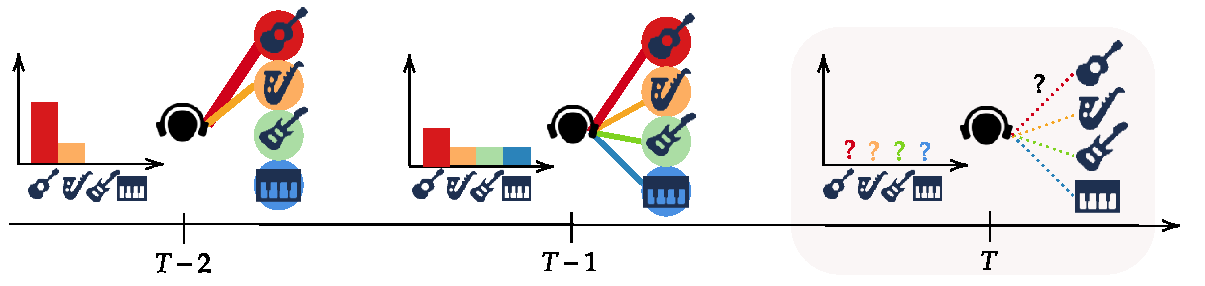
\includegraphics[width=0.8\textwidth]{figs/nodeproppred.pdf}} %\vspace{-15pt}
        \caption{\changed{The \emph{node affinity prediction} task aims to predict how the preference of a user towards items change over time.
        In the \fm example, the task is to predict the frequency at which the user would listen to each genre over the next week given their listening history until today. }}
        % https://www.mathcha.io/editor/lYlp6FlJTENfB1S7ojn1Zf6GDqBnuB3meyOu6PDwZ9
        \label{Fig:nodepred}
    \end{center}
    \vspace{-15pt}
\end{figure*}


% \textcolor{green}{[FP: what about having a drawing to better show what this task is?\\ here's a drawing: \href{https://www.mathcha.io/editor/DLlOvtVLFQ0H9OHLyPOYXt040J5efLVm6lJtWXGBZV}{nodeproppred}]}
% \ah{add example figure to show how to visualize the task, maybe a histogram of the node label, visualization the frequency interaction of lastgmgenre}

% In real world applications, it is often important to provide personalized recommendations for a user. In this way, it is often important to take a node centric view to model future interactions. The goal of this task is to predict the interactive pattern of a given node towards a set of specified nodes in the graph over a future period. For example, in the \fm dataset where we have the interaction history between users and different music genres. The node affinity prediction task then aims to predict the interaction frequency distribution of a given user towards a list of genres in the next week. 

%\gr{isn't this the only kind of property we consider in the \name datasets? If this is indeed the case you can rephrase as "In \name, we consider tasks where the property to predict is the distribution of a node's interactions with a given subset of nodes."}

% \ah{explain the task concretely for each dataset, explain the last fm genre as example here}

The goal of \emph{dynamic node property prediction} is to predict the property of a node \changed{at any given timestamp $t$, i.e., to learn a function $f:\mathbf{V}_t \to \mathcal{Y}$, where $\mathbf{V}_t$ is the set of nodes at time $t$ and $\mathcal{Y}$ is some output space~(e.g. $\{-1,+1\}$, $\mathbb{R}$, $\mathbb{R}^p$, etc). This is a general category for node level tasks such as node classification and node regression. Here, the property of the node can be a one hot label, a weight vector or an euclidean coordinate. 
Currently, there is a lack of large scale temporal graph datasets with node labels in the literature; therefore, we first include the \emph{node affinity prediction} task (as defined below). In the future, we will add more node level tasks and datasets into \name. }
%lack of large scale dataset
%the 

\changed{ \textbf{Node affinity prediction.} This task considers the affinity of a subset of nodes~(representing, e.g., users) towards other nodes~(e.g. items) as its property, and how the affinity naturally change over time.
This task is relevant for example in recommendation systems, where it is important to provide personalized recommendations for a user by modelling the their preference towards different items over time.}
Figure~\ref{Fig:nodepred} shows the node affinity prediction task in the context of music recommendation systems as seen in the \fm dataset. 
In this task, we are given the interaction history of a user with different music genres, and the goal is to predict the frequency at which the user would listen to each genre over the next week.

% predict the frequency of this user's interactions with different music genres over the next week. 
%how the node labels are generated 
%metric for node prop pred
More formally, given the observed evolution history of a temporal graph $\mathcal{G}_t$ until current timestamp $t$, the \changed{\emph{node affinity prediction}} task (on a dataset such as \fm) predicts the interaction frequency vector $\Vec{y}_t[u,:]$ for a node $u$ over a set of candidate nodes $\mathbf{N}$ within a fixed future period $[t,t+k]$ where $k$ is the window size defined by the application. 
Each entry in $\Vec{y}_t[u,:]$ corresponds to a candidate node $v \in \mathbf{N}$ and the groundtruth value is generated as follows:
% \begin{equation}
%     \Vec{y}_t[i] = \frac{ \sum_{t^* = (t+1)}^{(t+k)} w_{u,i,t^*}}{\sum_{i \in \mathbb{N}} \sum_{t^* = (t+1)}^{(t+k)} w_{u,i,t^*}}
% \end{equation}
% where $w_{u,i,t^*}$ is the weight of the edge $(u,i,t^*)$.
%\gr{\textit{This definition of $\Vec{y}_t$ is not consistent with the notation used when introducing dynamic graphs as edge streams. Here is a way to address this:} }
% \begin{align*}
\begin{equation}
    \Vec{y}_t[u,v] = \frac{ \sum_{ t < t_i \leq t+k} w_{(u,v,t_i)}}{\sum_{z \in \mathbf{N}} \sum_{ t < t_i \leq t+k} w_{(u,z,t_i)}}
\end{equation}
% \end{align*}
where $w_{(u,v,t_i)}$ is the weight of the edge $(u,v,t_i)$~(which we assume to be $0$ if the edge between $u$ and $v$ is not present at time $t_i$).
Observe that, by definition, $\|\Vec{y}_t[u,:]\|_1 = 1$. 
We use the Normalized Discounted Cumulative Gain~(NDCG) metric that takes into account the relative order of elements.
NDCG is commonly used in information retrieval and recommendation systems as a measure of ranking quality~\cite{jarvelin2002cumulated}. 
In this work, we use NDCG@10 where the relative order of the top 10 ranked items (\emph{i.e.} destination nodes) are examined. 
Specifically in the \fm dataset, the NDCG@10 compares the ground truth to the relative order of the top-10 music genres that a model predicts. 
%In this task, we care about the frequency ranking of the top candidate nodes. 
% \wh{This sounds like link prediction where the number of target nodes is not so large... Didn't we include churn prediction?}



% Node Prop Pred
% \begin{itemize}
%     \item Average review of a product in the next month, for node prop pred
%     \item stablecoin, the number of transactions in next month, average number of transactions in next month
%     \item US public twitter dataset, if the user will be viral, how many mentions, retweet the user will get? how influential a user is?! could be a measure of influence? 
%     15k nodes, 10-15 million edges, duration: 5 months, text embedding on the tweets
% \end{itemize}

